% Options for packages loaded elsewhere
\PassOptionsToPackage{unicode}{hyperref}
\PassOptionsToPackage{hyphens}{url}
\PassOptionsToPackage{dvipsnames,svgnames,x11names}{xcolor}
\documentclass[
  11pt,
  a4paper,
]{article}
\usepackage{xcolor}
\usepackage[margin=23mm]{geometry}
\usepackage{amsmath,amssymb}
\setcounter{secnumdepth}{-\maxdimen} % remove section numbering
\usepackage{iftex}
\ifPDFTeX
  \usepackage[T1]{fontenc}
  \usepackage[utf8]{inputenc}
  \usepackage{textcomp} % provide euro and other symbols
\else % if luatex or xetex
  \usepackage{unicode-math} % this also loads fontspec
  \defaultfontfeatures{Scale=MatchLowercase}
  \defaultfontfeatures[\rmfamily]{Ligatures=TeX,Scale=1}
\fi
\usepackage{lmodern}
\ifPDFTeX\else
  % xetex/luatex font selection
  \setmainfont[BoldFont=texgyrepagella-bold.otf,ItalicFont=texgyrepagella-italic.otf,BoldItalicFont=texgyrepagella-bolditalic.otf]{texgyrepagella-regular.otf}
  \setmonofont[]{lmmono10-regular.otf}
  \setmathfont[]{texgyrepagella-math.otf}
\fi
% Use upquote if available, for straight quotes in verbatim environments
\IfFileExists{upquote.sty}{\usepackage{upquote}}{}
\IfFileExists{microtype.sty}{% use microtype if available
  \usepackage[]{microtype}
  \UseMicrotypeSet[protrusion]{basicmath} % disable protrusion for tt fonts
}{}
\makeatletter
\@ifundefined{KOMAClassName}{% if non-KOMA class
  \IfFileExists{parskip.sty}{%
    \usepackage{parskip}
  }{% else
    \setlength{\parindent}{0pt}
    \setlength{\parskip}{6pt plus 2pt minus 1pt}}
}{% if KOMA class
  \KOMAoptions{parskip=half}}
\makeatother
\usepackage{longtable,booktabs,array}
\usepackage{caption}
\captionsetup[table]{skip=6pt}
\newcounter{none} % for unnumbered tables
\usepackage{calc} % for calculating minipage widths
% Correct order of tables after \paragraph or \subparagraph
\usepackage{etoolbox}
\makeatletter
\patchcmd\longtable{\par}{\if@noskipsec\mbox{}\fi\par}{}{}
\makeatother
% Allow footnotes in longtable head/foot
\IfFileExists{footnotehyper.sty}{\usepackage{footnotehyper}}{\usepackage{footnote}}
\makesavenoteenv{longtable}
\usepackage{graphicx}
\makeatletter
\newsavebox\pandoc@box
\newcommand*\pandocbounded[1]{% scales image to fit in text height/width
  \sbox\pandoc@box{#1}%
  \Gscale@div\@tempa{\textheight}{\dimexpr\ht\pandoc@box+\dp\pandoc@box\relax}%
  \Gscale@div\@tempb{\linewidth}{\wd\pandoc@box}%
  \ifdim\@tempb\p@<\@tempa\p@\let\@tempa\@tempb\fi% select the smaller of both
  \ifdim\@tempa\p@<\p@\scalebox{\@tempa}{\usebox\pandoc@box}%
  \else\usebox{\pandoc@box}%
  \fi%
}
% Set default figure placement to htbp
\def\fps@figure{htbp}
\makeatother
\setlength{\emergencystretch}{3em} % prevent overfull lines
\providecommand{\tightlist}{%
  \setlength{\itemsep}{0pt}\setlength{\parskip}{0pt}}
\usepackage{mathtools,graphicx,needspace,xurl,etoolbox,fancyhdr,titlesec}
\setlength{\parindent}{0pt}
\setlength{\parskip}{5pt plus 1pt minus 1pt}
\setlength{\emergencystretch}{2em}
\clubpenalty=10000
\widowpenalty=10000
\displaywidowpenalty=10000
\raggedbottom
\pagestyle{fancy}
\fancyhf{}
\fancyhead[L]{\scriptsize Historical TORMENT and the Trioctagon Physics Kernel}
\fancyhead[R]{\scriptsize REPOSITORY EDITION v0.1}
\fancyfoot[C]{\small\thepage}
\setlength{\headheight}{14pt}
\renewcommand{\headrulewidth}{0.2pt}
\titleformat{\section}{\normalfont\Large\bfseries}{}{0pt}{}
\titlespacing*{\section}{0pt}{15pt plus 3pt minus 2pt}{6pt}
\pretocmd{\section}{\Needspace{6\baselineskip}}{}{}
\pretocmd{\subsection}{\Needspace{5\baselineskip}}{}{}
\makeatletter
\renewenvironment{figure}[1][]{\par\noindent\begin{minipage}{\linewidth}\def\@captype{figure}}{\end{minipage}\par\medskip}
\def\@maketitle{\newpage\null\begin{center}{\LARGE\bfseries\@title\par}\vskip .9em{\large\@author\par}\vskip .5em{\small\@date\par}\end{center}\vskip .4em}
\makeatother
\newsavebox{\papereqbox}
\newcommand{\paperdisplay}[2][]{\par\begingroup
\sbox{\papereqbox}{$\displaystyle #2$}
\typeout{PAPER-EQUATION-WIDTH: \the\wd\papereqbox; available \the\linewidth; tag #1}
\begin{equation*}\ifdim\wd\papereqbox>.94\linewidth
\resizebox{.94\linewidth}{!}{\usebox{\papereqbox}}\else\usebox{\papereqbox}\fi
\ifstrempty{#1}{}{\tag{#1}}\end{equation*}\endgroup\par}
\usepackage{bookmark}
\IfFileExists{xurl.sty}{\usepackage{xurl}}{} % add URL line breaks if available
\urlstyle{same}
% fallback for those not using the hyperref driver hyperxmp:
\makeatletter
\@ifundefined{xmpquote}{\newcommand{\xmpquote}[1]{#1}}{}
\makeatother
\hypersetup{
  pdftitle={Historical TORMENT and the Trioctagon Physics Kernel: Lineage{,} Mathematical Equivalence{,} and Structural Divergence},
  pdfauthor={Hilmir Frímann Halldórsson},
  colorlinks=true,
  linkcolor={MidnightBlue},
  filecolor={Maroon},
  citecolor={Blue},
  urlcolor={MidnightBlue},
  pdfcreator={LaTeX via pandoc}}

\title{Historical TORMENT and the Trioctagon Physics Kernel: Lineage, Mathematical Equivalence, and Structural Divergence}
\author{Hilmir Frímann Halldórsson}
\date{1 October 2026 \textbar{} v0.1 REPOSITORY PUBLICATION}

\begin{document}
\maketitle

\textbf{Publication status.} Scientifically and editorially accepted by the author for repository publication. Prepared with Codex AI assistance in source review, drafting, data extraction and typesetting. This is not Paper G and has not been externally peer reviewed. No DOI is claimed.

\section{Abstract}\label{abstract}

Historical TORMENT and the current Trioctagon Physics kernel share a deterministic complex triad recurrence, but their names encompass different implementations, parameter policies and surrounding systems. We reconstruct that relationship from the H0-H6B audits and contract records and the P3 independent-kernel comparison. The accepted recurrence equivalence follows algebraically from the three-node coupling and simultaneous harmonic-three phase update. Separately, P3 records exact binary64 agreement for 75 successful matched one-step cases and 76,800 matched updates in pinned numerical environments. Those results concern an admitted unforced common domain, not whole production TORMENT. Historical scaled coefficients produce different amplitudes, transient separation and auxiliary memory drive from the current L01 unit-coefficient reference; the current kernel reproduces those measured behaviors when supplied the Historical coefficients. Historical 3D constructions did exist, but the recovered evidence does not establish that a folded C01-like shell drove production state updates. We distinguish source lineage, runtime coupling, mathematical equivalence and finite numerical agreement, and identify the Historical probability chart, initialization conventions and current structural extensions that remain outside simple recurrence parity. Neither physical validation nor an AI-memory winner follows from this comparison.

\section{1. Which kernels are being compared?}\label{which-kernels-are-being-compared}

Three identities are essential. \textbf{Production TORMENT} is the AI-memory application and its kernel inside the production repository, with service state, wrappers and interfaces. The \textbf{Historical TORMENT reference} is the clean independent distribution \nolinkurl{trioctagon-historical-kernel} 0.1.0, imported as \nolinkurl{trioctagon_historical_kernel}. The \textbf{current physics kernel} is \texttt{trioctagon-physics} 0.1.0, imported as \texttt{kernel\_physics}. The archived \texttt{kernel\_TO} tree is source evidence for historical mathematics; it is neither the complete production system nor the new Historical reference. {[}H2, H5, H6B{]}

The Historical reference implements selected equations and behavior frozen by H4/H5. The user-directed H5 amendment superseded H4\textquotesingle s proposed reuse of current scientific functions: the reference must implement its mathematics independently and import neither the current scientific functions nor archived historical code at runtime. Shared non-scientific codec and validation infrastructure does not make one kernel the other\textquotesingle s scientific implementation. Consequently, equality can be tested between two implementations of the same law. It is not established by having both call the same recurrence. {[}H5 §1; H6B §§5-17{]}

The repository baseline for this paper is commit \nolinkurl{9c9e579e97aac0cdc7524b0d05430d0d76e39ce4}. H6B\textquotesingle s independent implementation was certified at \nolinkurl{31109632fb1bb179a0f35f367f26f7472865a7b2}; P3 binds the compared installed distributions and verifies their scientific members against the accepted sources. These identities specify the comparison, not the provenance of every production behavior. Production itself was not rerun or modified for this paper.

\begin{figure}
\centering
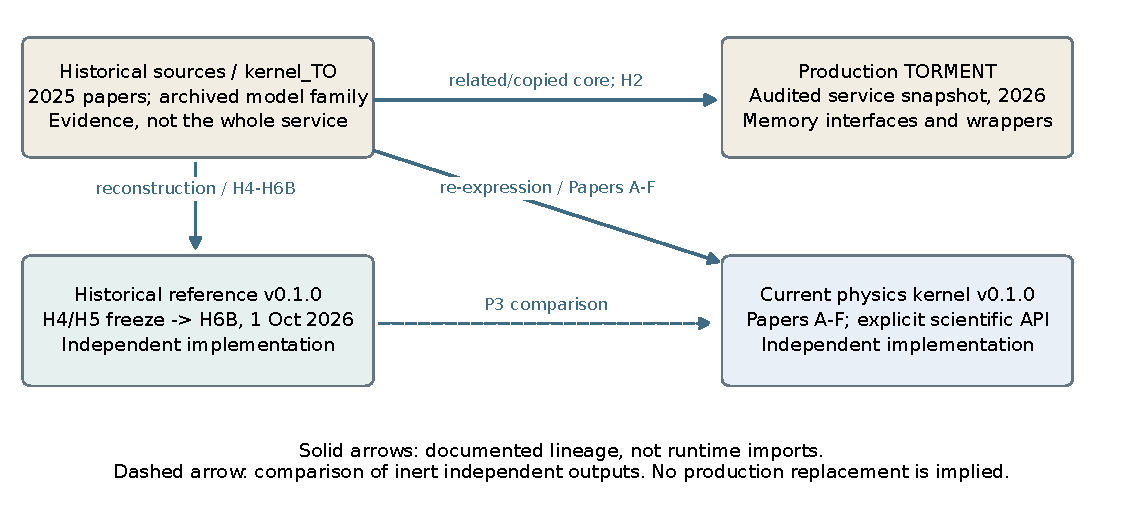
\includegraphics[width=1\linewidth,height=\textheight,keepaspectratio,alt={Documented lineage and comparison roles. Solid arrows summarize source relationships and reconstruction; they are not runtime import arrows. The independent reference was formalized after substantial current-kernel research already existed. P3 compares its outputs with current outputs and does not replace production TORMENT. Sources: H0-H6B and Papers A-F.}]{../figures/01_lineage.pdf}
\caption{Documented lineage and comparison roles. Solid arrows summarize source relationships and reconstruction; they are not runtime import arrows. The independent reference was formalized after substantial current-kernel research already existed. P3 compares its outputs with current outputs and does not replace production TORMENT. Sources: H0-H6B and Papers A-F.}
\end{figure}

\subsection{1.1. A dated, qualified lineage}\label{a-dated-qualified-lineage}

The retained 21 November 2025 \emph{Emergent Z} text contains a single-orientation threefold potential and normalized height bands. It is a precursor, with different variables from the later pairwise phase synchronizer. A December 2025 v3.9 paper documents harmonic-three pairwise coupling; its 29 December PDF build date is not proof of the date of invention. Production Git commit \nolinkurl{f462b312809996ea96bff382adddf37b5b0fa596}, dated 8 March 2026, attests the phase helper\textquotesingle s presence in that tree. It is a copy-in boundary, not recovered evidence of the original design decision. {[}H3 §§2-5{]}

An August 2026 passive A/B/C shell viewer and a September welded-shell reconstruction supply different geometry evidence. The 20 September edge-one reconstruction is a direct ancestor of current C01\textquotesingle s width-one construction. H0-H3, dated 30 September, separated these strands. H4 completed on 1 October, followed by H5, H6A and H6B\textquotesingle s independent protocol and mathematical implementation, and P3\textquotesingle s comparison. These are reconstruction and comparison milestones; they should not be projected back as historical author intent. The original discussion choosing the phase harmonic and several tuning constants has not been recovered. {[}H0, H1, H3-H6B{]}

\section{2. Geometry: existence, display and dynamical use}\label{geometry-existence-display-and-dynamical-use}

H0 did not identify a complete folded three-octagon shell specification in the audited production source. H1 expanded the provenance search and demonstrated that historical 3D constructions and displays nevertheless existed. Together they support a narrower conclusion: a C01-like folded shell has not been shown to drive the production \(\Omega\) recurrence. They do not establish that historical geometry was absent or universally irrelevant. {[}H0 §§1-6; H1 §§5-11{]}

Recovered \texttt{kernel\_TO} material contains cylinder/clock-Z trajectories, a torus fitted to trajectory history, three channel anchors separated by 120 degrees, and a fixed torus with major radius 2 and minor radius 0.6. It also includes dual tetrahedra: eight vertices do not make an octagonal face. The old torus viewer maps its local model state to coordinates and trails. The recovered path does not establish live binding to the production service or a reverse path from that mesh\textquotesingle s coordinates into \(\Omega\). Normalized 0.3/0.6/0.9 height bands in \emph{Emergent Z} are not evidence that those numbers were the radii of a three-ring shell. {[}H1 §§5-9{]}

Supplementary Three.js material constructs lifted eight-node loops and ribbons. The August passive shell candidate uses separate A/B/C loops or discs with 24 frame vertices, rather than C01\textquotesingle s 18 welded vertices. These can be conceptual ancestors without being geometrically equivalent meshes. Some earlier chamber-document references name \texttt{tri.py}, \texttt{center3.py}, \texttt{center2.py} and \texttt{david.png}; their original renderers were not recovered. A unique old solid or coordinate registration cannot be inferred from the prose alone. {[}H1 §§6-8{]}

Conversely, some production geometry-related calculations do have a traced consumer. The source audit follows a two-dimensional corridor map,

\paperdisplay[1]{Q(q,\kappa)=\bigl((2+\rho\cos\theta)\cos\theta,\ (2+\rho\cos\theta)\sin\theta\bigr),\qquad \rho=\frac{\kappa}{1+\kappa},}

through chart increments and monitors to write, proposal and bridge decisions. There are also external three-dimensional seed positions. This is evidence of service-level consumers in the inspected call paths, not evidence of C01 shell feedback or of every deployed execution. In particular, the unforced recurrence compared below receives no shell coordinates. {[}H1 §7.9; H2 §§16-18{]}

Current C01 is an explicit construction: three zero-thickness regular octagonal panels of flat-to-flat width 1, side length \(\sqrt2-1\), and fold \(\beta=\pi/3\) from a reversed stacked start. Welding produces 18 vertices, 21 edges and three faces, with three seams and two open nine-edge rims. Its surface is an annulus, not a filled solid torus; the axis-aligned bounding box is \(1\times\sqrt3/2\times1\) in the documented frame. The conversion from the September edge-one reconstruction to width one is the exact scale \(\sqrt2-1\). It is not an experimentally calibrated conversion from the older torus to C01. {[}H0; Paper C, construction and incidence sections{]}

Papers A-C separate the recurrence and its cycle-covering extension, channel-pair chirality and the folded construction. Paper D\textquotesingle s reference scaffold is a further specified geometric object, not a recovered production boundary. Mathematical construction, display geometry and recurrence input must therefore remain separate claims. Neither old torus coordinates nor current exact geometry supply physical units or an automatic spatial interpretation of the complex triad.

\section{3. The shared recurrence and its hypotheses}\label{the-shared-recurrence-and-its-hypotheses}

Let \(\Omega=(\Omega_1,\Omega_2,\Omega_3)\in\mathbb C^3\) be the ordered, raw complex state; \(k=(k_1,k_2,k_3)\) the real onsite coefficients; \(\epsilon=0.05\) the onsite step coefficient; \(g=0.2\) the graph coefficient; and \(\lambda=0.001\) the phase strength. Historical-v1 admits only the three literal \(k\) profiles in Section 4. The current comparison explicitly supplies those same values. Define the negative graph Laplacian

\paperdisplay[2]{L_3=\begin{pmatrix}-2&1&1\\1&-2&1\\1&1&-2\end{pmatrix}.}

The pre-phase state \(V\) and completed update \(F_k(\Omega)\) are

\paperdisplay[3]{V=\Omega+\epsilon\,\Omega\odot(k-|\Omega|^2)+gL_3\Omega,}

\paperdisplay[4]{\phi_j=\operatorname{Arg}_0(V_j),\qquad
F_k(\Omega)_j=|V_j|\exp\!\left(i\left[\phi_j+\lambda\sum_{\ell\ne j}\sin\bigl(3(\phi_\ell-\phi_j)\bigr)\right]\right).}

Here \(\odot\) and \(|\Omega|^2\) act componentwise, \(i^2=-1\), and \(\operatorname{Arg}_0\) sets the phase of every exact complex zero to positive zero. All terms of (3) use the same old state. All phase differences in (4) use the original pre-phase angles, simultaneously. The sign is neighbor minus own angle. The coupling coefficient is \(g\), not \(\epsilon g\). There is no additional time-step factor, state normalization, forcing, noise or observer feedback. {[}H2 §§6,9-11; H4 §4; H5 §1{]}

The notation correspondence is direct: historical \texttt{eps}, \texttt{g}, \texttt{k\_vals} and \texttt{lambda\_phase} map to current \texttt{eps}, \texttt{g}, \texttt{k} and \texttt{phase\_strength}. Historical clock fields and readout coefficients map separately to current observer configuration. Older source options for additive forcing before synchronization and noise afterward are excluded; their existence does not broaden the Historical reference API.

\subsection{3.1. Algebraic equivalence is not a test count}\label{algebraic-equivalence-is-not-a-test-count}

On three nodes, the two cyclic neighbors are exactly the other two nodes. Their differences sum to \(\Omega_{j-1}+\Omega_{j+1}-2\Omega_j\), the \(j\)th component of \(L_3\Omega\). Thus the historical graph term and current cycle formulation agree; the current triad implementation evaluates this matrix product directly. The onsite terms also agree componentwise, giving the same mathematical \(V\). The two neighbor phase contributions in the current form equal the sum over \(\ell\ne j\) in (4); including a self-term would add only \(\sin0=0\). Matched angle conventions therefore give the same map. By induction, equal initial states and fixed matched parameters give equal ideal mathematical trajectories. {[}H2 §§4-6,9{]}

This proof is qualified at the implementation boundary. Some archived helpers used \texttt{np.angle} directly and did not canonicalize signed complex zero. H2 recovered an actual helper-level counterexample; H4/H5 explicitly adopt the canonical-zero convention, rather than claim every old helper already had it. Branch cuts, arithmetic association and library evaluation also prevent turning an algebraic identity into a theorem about all binary64 executions. Common-phase equivariance statements need nonzero phase-chart qualifications at zero-amplitude strata. {[}H2 §9; H6B §17{]}

We therefore distinguish: \textbf{(i)} the accepted algebraic equality under these hypotheses; \textbf{(ii)} the exact numerical equality measured for particular implementations and inputs in P3; and \textbf{(iii)} equality of whole production systems, all parameter regimes or physical phenomena, which neither establishes. The current kernel\textquotesingle s larger rings have additional states. A three-periodic lift into a ring of length divisible by three intertwines the matching maps, but does not make every ring state equivalent to a triad. {[}Paper A §§1,6; H2; P3 §§5,17{]}

\section{4. Historical tuning and the role of harmonic three}\label{historical-tuning-and-the-role-of-harmonic-three}

The scaled Historical profile is the recorded historical default. L01 is a selected current reference scenario, not a universal current API default. Their constants are:

{\def\LTcaptype{none} % do not increment counter
\begin{longtable}[]{@{}ll@{}}
\toprule\noalign{}
Profile & Exact decimal coefficient literals \((k_1,k_2,k_3)\) \\
\midrule\noalign{}
\endhead
\bottomrule\noalign{}
\endlastfoot
Historical scaled & \((1,\ 1.2208964704604097,\ 6.35310346037241)\) \\
Historical soft & \((1,\ 1.104941840306724,\ 2.52053634379122)\) \\
Historical simple & \((0.7,\ 1,\ 1.3)\) \\
Current L01 & \((1,\ 1,\ 1)\) \\
\end{longtable}
}

The admitted identifiers are \nolinkurl{HISTORICAL_THETA_SCALED}, \nolinkurl{HISTORICAL_THETA_SOFT} and \texttt{HISTORICAL\_SIMPLE}. They freeze values; they do not expose a selector. In the recovered selector\textquotesingle s provenance, with \(\varphi=(1+\sqrt5)/2\),

\paperdisplay[5]{\vartheta(a,b)=\frac{|a/b-b/a|}{\sqrt{ab}},\qquad
h=\bigl(\vartheta(\sqrt3,\varphi),\vartheta(\pi,e),\vartheta(\varphi,e)\bigr).}

The scaled values came from \(h/h_1\); soft used the componentwise square root with scale coefficient 1. Equation (5) documents the selection procedure, not a physical derivation or proof of optimality. The surviving evidence reconstructs how these coefficient values were calculated, but not why the particular constant pairs \((\sqrt3,\varphi)\), \((\pi,e)\), and \((\varphi,e)\) were originally chosen. The selector symbol \(\vartheta\) is unrelated to a phase or readout clock angle. Its ratio construction does not provide a uniform change of amplitude units that turns unequal \(k_j\) into three unit coefficients: \(\Omega=sY\) changes the onsite coefficients to \(\epsilon s^2\) and \(k/s^2\), preserving unequal ratios. {[}H2 §7; H4 §5; P3 §§6-7{]}

The multiplier 3 in (4) has a different role from the number of state channels, three-dimensional display coordinates, three height labels or a 12-sector clock. Channel permutations and a common phase shift, where the phase chart is defined, do not uniquely select harmonic three. H3 found a conditional rationale: if one assumes independent identification of each phase under a 120-degree shift, allowed integer pairwise harmonics are multiples of three. Selecting the lowest nonconstant pure harmonic then makes three natural. That premise is an additional modeling choice; independent rephasing is not a symmetry of the full graph-coupled amplitude step when \(g\ne0\). {[}H3 §§6-9{]}

H3 also corrects a factor omitted in the old potential argument. For a pair potential

\paperdisplay[6]{U=A\sum_{j<\ell}\bigl[1-\cos\bigl(3(\phi_\ell-\phi_j)\bigr)\bigr],}

a gradient step with step size \(\eta\) has the positive phase increment in (4) with \(\lambda=3\eta A\), not \(\eta A\). This is a mathematical qualification of the derivation, not a proposal to rescale the frozen coefficient. The historical motivation for that specific choice is incompletely documented. Three is a supported historical model choice, not a constant compelled by three channels or validated by physics.

\section{5. Z, chirality and auxiliary memory}\label{z-chirality-and-auxiliary-memory}

The recurrence evolves \(\Omega\); observers consume it. Let \(\kappa\) be the Euclidean norm of its six real coordinates, \(q\) a sector index, \(t\) the observer time, and \(m\) the auxiliary exponential-moving-average (EMA) memory. For the compared historical settings,

\paperdisplay[7]{\rho=\frac{\kappa}{1+\kappa},\qquad
\theta=\frac{2\pi(q\bmod12)}{12},\qquad
H(\Omega,q)=0.618\rho\cos\bigl(3(\theta-0.244)\bigr).}

The observer angle \(\theta\) is not any component angle \(\phi_j\). Staged K and cognitive EMA H are distinct laws:

\paperdisplay[8]{z_K=H(\Omega,q)e^{-0.577t},\qquad
z_H=H(\Omega,q)+m.}

EMA advancement, once per newly updated state, is

\paperdisplay[9]{J=\Im\bigl((\Omega_1\overline{\Omega_2})\Omega_3\bigr),\qquad
m^+=0.99m+0.01\frac{J}{1+|J|}.}

Detached EMA inspection reads the supplied current \(m\) and never advances it. The 0.01 innovation is a literal, not the binary64 expression \texttt{1\ -\ float(.99)}. Likewise 0.618, 0.244 and 0.577 are the recorded decimal constants, not substituted exact values of a golden ratio, guessed angle or Euler constant. No staged envelope multiplies \(z_H\). {[}H2 §§12-13; H4 §§8-10; Paper E{]}

For either selected scalar \(z\), the macro vector, chirality and historical blend are

\paperdisplay[10]{M=z(\cos\theta,\sin\theta,1),\qquad
C=\bigl(\Im(\overline\Omega_2\Omega_3),\Im(\overline\Omega_3\Omega_1),\Im(\overline\Omega_1\Omega_2)\bigr),}

\paperdisplay[11]{C=\Re\Omega\times\Im\Omega,\qquad T=M+0.5C.}

Current configurable \(T=\alpha M+\beta C\) matches at \((\alpha,\beta)=(1,0.5)\). Raw \(C\) is quadratic in amplitude and invariant under common phase rotation; it is not a normalized direction. The cubic \(J\) is a different observable and can change under that rotation. Paper B interprets the components of \(C\) as signed channel-pair state-vector areas. Neither the algebraic cross product nor the name ``chirality'' automatically registers it as a physical Cartesian vector on a historical shell. The staged exponential acts on \(z_K\), not on raw \(C\) or \(\Omega\). {[}Paper B §§6-8; H2 §13{]}

Production also contains distinct core-staged and cognitive uses of ``Z''; the cognitive scalar is not simply substituted into every core vector. Agreement of a named formula does not prove agreement of all service consumers. The Historical and current strict response implementations use checked products, stable norms and compensated sums; their successful domain excludes some subnormal or underflowed intermediate values. This policy differs both from raw recurrence arithmetic with gradual underflow and from the legacy probability chart. {[}H2 §12; H5; H6B §§9-13{]}

\subsection{5.1. Initialization, clocks and history alignment}\label{initialization-clocks-and-history-alignment}

Fresh Historical runs begin with \(q=0\), \(t=+0\) and \(m=+0\), and literal zero cached \(z,M,C,T\), even when a detached formula evaluation at the same \(\Omega\) would be nonzero. Each update advances \(\Omega\), then \(q\mapsto(q+1)\bmod12\) and repeated binary64 \(t\mapsto t+0.1\), then selected EMA memory once from new \(\Omega\), then the observation. This clock is downstream of the recurrence. {[}H4 §7; H6B §10{]}

For \(N\) updates the Historical result stores \(N\) pre-update rows plus a separate terminal; the current run stores its initial sample plus \(N\) updated samples. Historical row \(j\) maps to current sample \(j\) for \(0\le j<N\), and the Historical terminal maps to sample \(N\). At \(N=0\), zero Historical rows and one constructor terminal correspond to one current initial sample. Current must explicitly choose constructor-zero observation; its named historical preset otherwise recomputes the initial observation. P3 tested 16 actual history mappings: staged/EMA times \(N=0,1,2,8,16,64,256,1024\). {[}P3 §15{]}

Computing \(t=N\times0.1\) is not equivalent to repeated binary64 addition. Already at \(N=8\), the respective hexadecimal values are \nolinkurl{0x1.999999999999ap-1} and \nolinkurl{0x1.9999999999999p-1}. Initial diagnostic observations in P3 were recomputed for formula comparison; that does not erase constructor-zero semantics in its separate history tests.

\section{6. P3 comparison design and measured agreement}\label{p3-comparison-design-and-measured-agreement}

P3 separated \textbf{Mode A}, matched coefficients in the two independent implementations, from \textbf{Mode B}, each Historical profile versus current L01. Both used \(\epsilon=0.05\), \(g=0.2\), \(\lambda=0.001\), harmonic three and matched admitted clocks and observer settings. The two installed execution environments were Windows x64, Anaconda CPython 3.11.15 and NumPy 2.4.4. Source/wheel binding and live import-denial checks supported implementation independence. Process isolation and installed-file identities did not establish protected execution attestation or certify production. {[}P3 §§2-5{]}

The 26 deterministic initial states comprised 13 inherited H2/H6B inputs and 13 additions. They include zero, isolated channels, equal real and complex-phase states, an approximate 120-degree pattern, asymmetric real and complex states, tiny and moderate amplitudes, near-sector pairs, radius-boundary cases, signed zeros, scaled and globally rotated seeds, and an overflow witness. This is an explicit finite sample, not a random population estimate. The three Historical profiles each see all 26 first-step inputs.

{\def\LTcaptype{none} % do not increment counter
\begin{longtable}[]{@{}
  >{\raggedright\arraybackslash}p{(\linewidth - 2\tabcolsep) * \real{0.5000}}
  >{\raggedright\arraybackslash}p{(\linewidth - 2\tabcolsep) * \real{0.5000}}@{}}
\toprule\noalign{}
\begin{minipage}[b]{\linewidth}\raggedright
P3 population
\end{minipage} & \begin{minipage}[b]{\linewidth}\raggedright
Count and outcome
\end{minipage} \\
\midrule\noalign{}
\endhead
\bottomrule\noalign{}
\endlastfoot
Matched first-step cases & \(3\times26=78\): 75 successful and exact; three joint overflow refusals \\
Matched trajectory pairs & \(3\times25=75\), excluding the overflow input \\
Updates and samples & \(75\times1024=76{,}800\) updates; 76,875 samples including initial states \\
Current L01 controls & 25 trajectories, used separately for coefficient contrast \\
Actual history mappings & 16 comparisons, exact under matched constructor policy \\
\end{longtable}
}

``Exact'' means equality of the compared finite binary64 hexadecimal tokens, including signed-zero identity where applicable: \(\Omega\), captured pre-phase state, clock \(q,t\), successful staged/EMA readouts and vector decompositions, chirality and memory. Refusal or unavailability status also matches. It does not require complete serialized artifacts, provenance or exception messages to be byte-identical. No unexpected shared-domain divergence was found. {[}P3 §§3,5,8-9,15{]}

Not every one of the 76,875 samples has a successful strict observation. There are 69,386 successful staged observations and 7,489 refusals; 64,578 successful EMA observations, 3,081 refusals and 9,216 unavailable observations; and 72,491 successful raw chirality observations and 4,384 refusals. Memory has 67,659 successful values, nine first-advance refusals and 9,207 subsequent unavailable values. Counts include recomputed diagnostic initial samples. The nine memory stops are three tiny-state inputs across three profiles, first at update 1. Their memory lanes are not reset or replaced by zeros. An external diagnostic trajectory may continue raw \(\Omega\) after an observer stops; an official run requesting that failed observer does not thereby become a successful run. {[}P3 §9{]}

H6B\textquotesingle s earlier H2 fixture coverage is a separate population: 39 of 91 one-step fixtures and 640 of 1,280 trajectory steps satisfy the frozen Historical-v1 parameter domain. Those were exact for the compared recurrence. H6B also compared 640 state/clock/readout/memory samples between the independent implementations. H2\textquotesingle s older source-to-current observer comparison included small nonzero rounding differences; it was not blanket bitwise observer parity. None of these counts is added to the P3 totals. {[}H2; H6B §§15-17{]}

\section{7. What changes when the coefficients change?}\label{what-changes-when-the-coefficients-change}

The first pre-phase difference between the Historical coefficients and L01, from a common state, is exactly the change in the onsite term,

\paperdisplay[12]{\Delta V=0.05\,\Omega\odot(k_{\rm Historical}-\mathbf1).}

This identifies the earliest causal difference without introducing a different recurrence. Starting at \((1,1,1)\), scaled Historical produces \((1,1.0110448235230205,1.2676551730186205)\) on the first step while L01 stays at \((1,1,1)\). For the first isolated channel, scaled \(k_1=1\) and the other components initially vanish: both first outputs are \((0.6,0.2,0.2)\), and divergence begins only on update 2. Zero remains zero. Thus not every input differs immediately. {[}P3 §8{]}

Figure 2 shows the frozen representative \texttt{gate\_seed},

\paperdisplay[13]{\Omega_0=(0.2+0.3i,\ -0.4+0.1i,\ 0.1-0.2i).}

It is one named example from the full population, not a summary of all initial states. The plots reuse P3\textquotesingle s saved outputs. Under matched Historical coefficients, current and Historical give identical measured trajectories; plotting both would overlay exactly. L01 instead uses the unit triple.

\begin{figure}
\centering
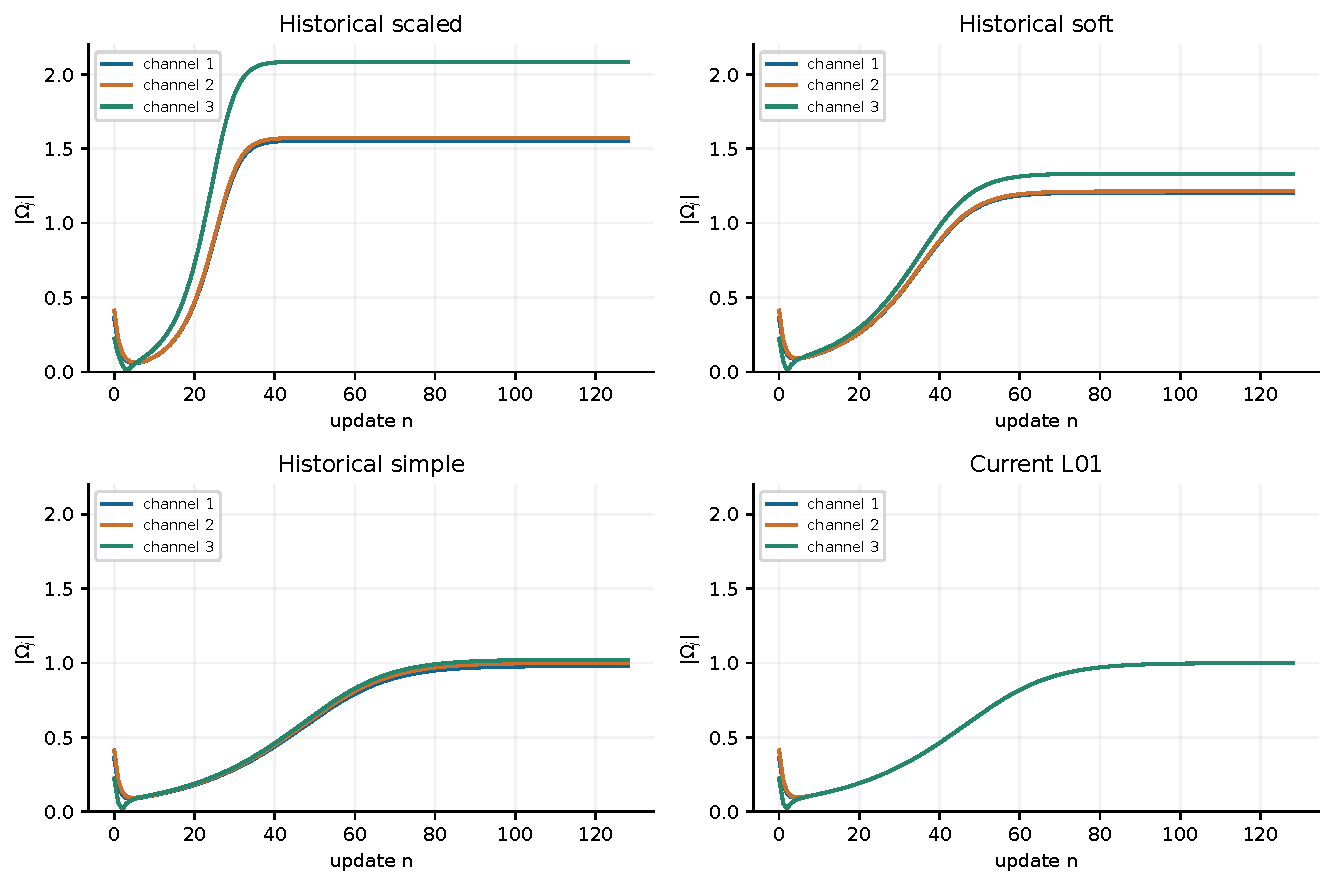
\includegraphics[width=1\linewidth,height=\textheight,keepaspectratio,alt={Coefficient-driven amplitude contrast for P3 gate\_seed (13). Each panel uses the profile in Section 4 with epsilon 0.05, graph coefficient 0.2 and phase strength 0.001. The plotted readouts are the three raw channel magnitudes through update 128, from saved 1024-update trajectories. Historical panels also describe the exactly matching current same-coefficient controls. The current L01 panel has coincident channel curves after its early transient. Source: P3 raw gate\_seed records.}]{../figures/02_amplitudes.pdf}
\caption{Coefficient-driven amplitude contrast for P3 gate\_seed (13). Each panel uses the profile in Section 4 with epsilon 0.05, graph coefficient 0.2 and phase strength 0.001. The plotted readouts are the three raw channel magnitudes through update 128, from saved 1024-update trajectories. Historical panels also describe the exactly matching current same-coefficient controls. The current L01 panel has coincident channel curves after its early transient. Source: P3 raw gate\_seed records.}
\end{figure}

At update 1024 the saved values are as follows, rounded here for readability; the local figure data retains the underlying values.

{\def\LTcaptype{none} % do not increment counter
\begin{longtable}[]{@{}llrr@{}}
\toprule\noalign{}
Configuration & Channel magnitudes & \(\|\Omega\|_2\) & EMA \(m\) \\
\midrule\noalign{}
\endhead
\bottomrule\noalign{}
\endlastfoot
Scaled & 1.554468, 1.573421, 2.085940 & 3.040258 & 0.816467 \\
Soft & 1.205126, 1.213402, 1.333129 & 2.168388 & 0.634243 \\
Simple & 0.980350, 1.001439, 1.023250 & 1.735225 & 0.468953 \\
L01 & 1.000000, 1.000000, 1.000000 & 1.732051 & 0.472442 \\
\end{longtable}
}

The scaled gate trajectory has larger channel imbalance and amplitude than L01, with soft and simple closer to L01 in this example. To separate common rotation from other changes, P3 reports both raw distance and aligned distance,

\paperdisplay[14]{d(x,y)=\|x-y\|_2,\qquad d_U(x,y)=\min_{\psi\in\mathbb R}\|e^{i\psi}x-y\|_2.}

The terminal raw/aligned pairs are 1.352280/1.347409 (scaled), 0.446378/0.445636 (soft), and 0.069106/0.030475 (simple). The scaled difference is therefore not merely a common phase rotation. Alignment is a comparison diagnostic, not a declaration that phase is physically unobservable or that a smaller distance is better memory.

\begin{figure}
\centering
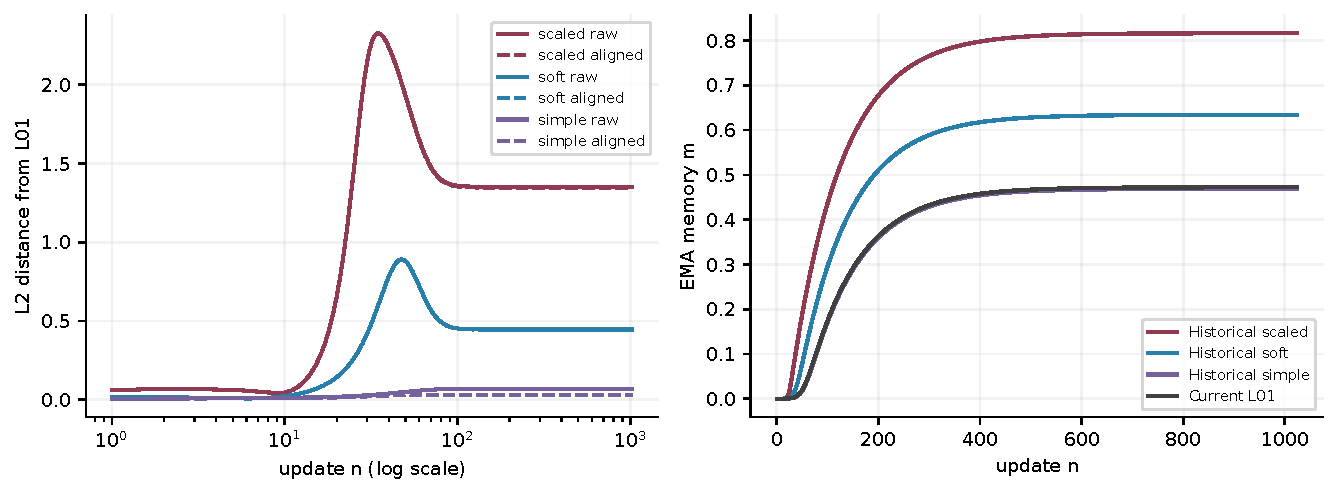
\includegraphics[width=1\linewidth,height=\textheight,keepaspectratio,alt={P3 gate\_seed through update 1024, with the same parameters as Figure 2. Left: raw distance (solid) and common-phase-aligned distance (dashed) from current L01, for each Historical profile. Only the update axis is logarithmic; the shared initial zero distance at n=0 is omitted from this log-x panel, not mapped to a positive error floor. Right: saved EMA memory from initial m=0, advanced once per updated state. Historical same-coefficient and current controls coincide exactly. Sources: P3 gate\_seed trajectories and metrics.}]{../figures/03_distance_memory.pdf}
\caption{P3 gate\_seed through update 1024, with the same parameters as Figure 2. Left: raw distance (solid) and common-phase-aligned distance (dashed) from current L01, for each Historical profile. Only the update axis is logarithmic; the shared initial zero distance at n=0 is omitted from this log-x panel, not mapped to a positive error floor. Right: saved EMA memory from initial m=0, advanced once per updated state. Historical same-coefficient and current controls coincide exactly. Sources: P3 gate\_seed trajectories and metrics.}
\end{figure}

Different transient diagnostics answer different questions. For the gate seed, P3\textquotesingle s first window of 32 increments below \(10^{-12}(1+\|\Omega\|_2)\) ends at updates 126, 216 and 315 for scaled, soft and simple. Those bounded indicators are not proofs of asymptotic convergence, and do not imply scaled always settles more slowly. Across the three isolated-channel starts, however, their maximum pairwise separation at update 16 is approximately 0.18116, 0.11067 and 0.03682 under those profiles, versus \(1.1755\times10^{-6}\) for L01. By update 1024 all four configurations have separation at most \(2.22\times10^{-16}\). Longer measured transient separation is not permanent retention of starting-channel identity. {[}P3 §§9-10{]}

All 25 non-overflow inputs per configuration remain finite through the 1024-update horizon. The near-sector probe shows modest terminal separation, not an established sector barrier, chaos or memory capacity. The radius probes include a deliberately just-outside case; these observations do not certify that every initial state lies in an optional operating region.

\subsection{7.1. Auxiliary memory is not a memory benchmark}\label{auxiliary-memory-is-not-a-memory-benchmark}

Equation (9) explains why different amplitudes and phases can alter EMA drive. P3\textquotesingle s globally \(i\)-rotated scaled gate seed has the same probability chart and common-phase-invariant chirality as its unrotated counterpart, yet its terminal memory is approximately \(-0.713921\), compared with \(0.816467\). The cubic \(J\) responds to phase information that the chart and \(C\) discard. Tiny terminal chirality therefore does not establish negligible EMA drive. {[}P3 §§12-14{]}

If two EMA memories subsequently receive exactly the same drive, their ideal homogeneous difference decays as \(0.99^n\), with a half-life of about 68.97 updates. A nonzero \(m\) under continuing drive is not by itself retention of a past event. This distinction applies to both implementations. Neither the amplitude table nor the EMA curve measures write/retrieval accuracy, useful delay, capacity or robustness for an AI-memory task.

\section{8. Structural differences beyond the shared law}\label{structural-differences-beyond-the-shared-law}

The Historical probability chart has no current numeric counterpart. With \(a_j=|\Omega_j|^2\), \(S=\sum_j a_j\), and \(w=a/S\) when \(S>0\) (otherwise \(w=a\)), its ordered coordinates are

\paperdisplay[15]{c=B^T w,\qquad
B=\begin{bmatrix}\dfrac{(1,1,1)^T}{\sqrt3}&\dfrac{(1,-1,0)^T}{\sqrt2}&\dfrac{(1,1,-2)^T}{\sqrt6}\end{bmatrix},\quad c=(c_u,c_x,c_y).}

For ordinary nonzero inputs this chart retains normalized intensity imbalance, discarding phase and common amplitude scale. Since \(c_u=1/\sqrt3\) in exact arithmetic, only two coordinates vary. A full chart artifact also stores intensities and their sum; the information loss just described concerns chart coordinates alone. Its frozen legacy numerical order is abs, square, sum, divide-if-positive, then basis multiplication. Tiny nonzero values whose squares underflow can yield the zero branch, with explicit flags; they are not silently replaced by a stabilized normalization. The lack of a current chart means \textbf{not comparable}, not zero output or a failed parity test. {[}H2 §14; H4 §11; H6B §13; P3 §14{]}

{\def\LTcaptype{none} % do not increment counter
\begin{longtable}[]{@{}
  >{\raggedright\arraybackslash}p{(\linewidth - 4\tabcolsep) * \real{0.3333}}
  >{\raggedright\arraybackslash}p{(\linewidth - 4\tabcolsep) * \real{0.3333}}
  >{\raggedright\arraybackslash}p{(\linewidth - 4\tabcolsep) * \real{0.3333}}@{}}
\toprule\noalign{}
\begin{minipage}[b]{\linewidth}\raggedright
Operation or structure
\end{minipage} & \begin{minipage}[b]{\linewidth}\raggedright
Historical reference
\end{minipage} & \begin{minipage}[b]{\linewidth}\raggedright
Current physics kernel
\end{minipage} \\
\midrule\noalign{}
\endhead
\bottomrule\noalign{}
\endlastfoot
Raw deterministic triad & Fixed constants; three literal \(k\) profiles & Same map when configured alike; broader explicit parameters \\
Staged/EMA and chirality & Frozen variants and strict domains & Matching passive observers; configurable decomposition \\
Initialization/history & Zero caches; pre-update rows plus terminal & Explicit initialization policy; initial plus updated samples \\
Probability chart & Reconstructed ordered chart, legacy underflow flags & No numeric counterpart \\
Larger rings & No Historical-v1 operation & Documented cyclic-ring extension; not all states reduce to triads \\
Exact geometry & No shell in the recurrence & Separate explicit constructions and geometry records \\
Other diagnostics & Selected historical operations only & Additional geometry/readout accounting; support varies \\
Production memory system & Excluded from the reference & Not reproduced by the scientific facade \\
\end{longtable}
}

Current separation of dynamics, clocks, passive observers and readouts makes scientific composition explicit; it is not evidence that the older core lacked those formulas. Current\textquotesingle s optional operating-region, boundary-response and SRG facilities remain under the repository\textquotesingle s Option B unsupported-public-v1 qualification, and face-state facilities are internal rather than part of the initial public facade. An optional radius-three operating profile does not impose a universal bound on every raw recurrence call. {[}Current kernel README; P3 §§17-19{]}

Historical production wrappers, gates, corridor monitors, labels, forcing/noise options, seed-world integration and the surrounding memory service are outside the independent reference\textquotesingle s five admitted operations. Record schemas, packaging and read-only UI access also differ, but do not establish a different scientific map. Independent implementation is valuable comparison evidence; it does not make the reference an oracle for deliberately excluded production behavior.

\section{9. Limits and practical consequences}\label{limits-and-practical-consequences}

The most specific supported conclusion is that the reconstructed unforced triad law survives, and that the two independently implemented versions agree exactly on the measured matched domain. Default-driven differences in P3 are reproducible by changing the current coefficients to the Historical values. This is stronger than a superficial similarity of plots and narrower than certification of whole applications.

The work is mathematical reconstruction and bounded numerical comparison, not experimental physical validation. No calibrated material, device, spatial units or measured physical prediction is supplied. The finite inputs and 1024-update horizons do not prove all-input, all-platform or infinite-time behavior. The production source snapshot, archived tree and independent reference have different coverage. The present paper neither re-executes historical code nor runs new kernel experiments.

Unresolved historical questions remain: the earliest harmonic-three design decision, the reasons for particular tuning literals, the missing original chamber renderers, and a demonstrated binding between a C01-like historical shell and production updates. A static service call path is not proof of every deployment. Shared terminology such as Z, torus or chirality cannot fill those gaps.

No AI-memory winner has been established. A meaningful comparison would require a specified encoding, task, delay, perturbation model, readout and success metric, with matched-coefficient controls kept separate from parameter-choice experiments. Longer separation on a few starts and nonzero EMA drive are candidate behaviors to study, not quality scores. Future physical interpretation likewise needs evidence beyond analogy.

The Historical reference can guide a later production-cleanup audit by supplying explicit, independent mathematical expectations. Such work must also preserve production behavior and interfaces beyond the reference\textquotesingle s coverage. This paper authorizes no cleanup or replacement. Author acceptance does not authorize production changes.

\section{10. Evidence access and reproducibility}\label{evidence-access-and-reproducibility}

This paper uses the accepted source basis specified by the 1 October work order: H0-H6B and P3. The reports retain their original review-stage wording; this manuscript does not retroactively edit those records or imply new external acceptance. Papers A-F are cited at the editions in the repository publication index. A compact companion \nolinkurl{evidence/SOURCE_MAP.md} maps equations, tables and major claims to exact report sections, code symbols or inert datasets, and distinguishes algebraic, numerical, documentary and unresolved support.

The repository bundle includes minimal derived figure/table data, source hashes, figure code and an editable Markdown manuscript with an isolated Pandoc/TeX build entry point. The figures use existing accepted P3 data; preparation checks record identities, counts and the selected trajectories without importing either kernel. Rebuilding this PDF from the included excerpt is distinct from independently reproducing P3\textquotesingle s scientific executions.

The underlying H/P3 packets, installed-wheel evidence and complete trajectory population remain local evidence, not a publicly accessible reproduction package. The source map identifies the minimum dependencies. The author has approved repository publication of this manuscript and its included derived excerpts and figures. That approval does not make the underlying local evidence public. The repository\textquotesingle s software license does not automatically license papers, research evidence or figures. Repository publication does not establish that the comparison is independently reproducible from a public checkout alone.

\section{References and source editions}\label{references-and-source-editions}

\textbf{{[}H0{]}} \emph{Historical/Current Geometry Equivalence Audit}, v0.1, 30 September 2026. Local primary audit.

\textbf{{[}H1{]}} \emph{Historical 3D Provenance \& Runtime-Binding Audit}, v0.1, 30 September 2026. Local primary audit, with explicit provenance limits.

\textbf{{[}H2{]}} \emph{Historical vs Current State/Dynamics Equivalence Audit}, v0.1, 30 September 2026. Local source comparison and bounded numerical evidence.

\textbf{{[}H3{]}} \emph{Harmonic-Three Derivation \& Provenance Audit}, v0.1, 30 September 2026. Local provenance and mathematical qualification.

\textbf{{[}H4{]}} \emph{Historical Compatibility Contract Freeze}, v0.1, completed 1 October 2026. Selected mathematical and behavioral contract; reuse proposals superseded as described by H5.

\textbf{{[}H5{]}} \emph{Historical Protocol \& Schema Admission Freeze}, v0.1, 1 October 2026, including the independent-kernel amendment. Implementation independence is controlling.

\textbf{{[}H6A{]}} \emph{Historical Protocol/Schema Implementation}, v0.1, 1 October 2026. Independent Historical protocol and schema record.

\textbf{{[}H6B{]}} \emph{Independent Historical Kernel Implementation}, v0.1, 1 October 2026. Implementation, conformance and scoped independent comparison; repository specification and conformance map accompany it.

\textbf{{[}P3{]}} \emph{Historical/Current Kernel Comparison Atlas}, v0.1, 1 October 2026, with \nolinkurl{p3_comparison_20261001} inert records. Primary finite-comparison dataset.

\textbf{{[}A{]}} Hilmir Frímann Halldórsson, Paper A, \emph{Cycle-Covering Dynamics of a Three-State Nonlinear Kernel}, publication v1.0 (scientific source v0.5.1). Recurrence and invariant ring reduction.

\textbf{{[}B{]}} Hilmir Frímann Halldórsson, Paper B, \emph{Triadic Chirality and Orientation Geometry}, v0.1.2. In particular, channel-pair area interpretation and its scope in Sections 6-8.

\textbf{{[}C{]}} Hilmir Frímann Halldórsson, Paper C, \emph{Exact Geometry of the Folded Tri-Octagon Module}, publication v1.0.1 (scientific source v0.3.1). Exact folded construction and incidence.

\textbf{{[}D{]}} Hilmir Frímann Halldórsson, Paper D, \emph{Tri-Octagon Reference-Scaffold Geometry: Exact Construction of an Alternating Hexagonal Core}, v0.1.1. Separate reference geometry and its declared relations.

\textbf{{[}E{]}} Hilmir Frímann Halldórsson, Paper E, \emph{The Tri-Octagon Z Manifold: Harmonic Macro Geometry, Chiral Deformation, and Diagnostic Dynamics}, v0.1.1. Staged/EMA observers and decomposition.

\textbf{{[}F{]}} Hilmir Frímann Halldórsson, Paper F, \emph{Transverse Chirality, Dihedral Harmonic Selection, and Local Linearization in a Three-Channel Nonlinear Map}, publication v0.2. Local dynamics, not a provenance derivation of the historical phase harmonic.

\textbf{Repository specifications.} \nolinkurl{historical_kernel/SPECIFICATION.md}, \texttt{CONFORMANCE.md} and \nolinkurl{tools/conformance_map.json}; \nolinkurl{kernel_physics/README.md}; \nolinkurl{scientific_domains/TORMENT_HISTORICAL.md}; and \texttt{LICENSE\_SCOPE.md}, at the baseline recorded in Section 1. Exact filenames and identities for all cited editions are in the companion source map.

\end{document}
